\section{Introductions}

Task Oriented Dialog(TOD) systems interact with users in the form of dialog using natural language, to accomplish user tasks.
The system needs to understand user needs and provide the best possible response to the user.
The task of extracting user intent and goals from conversations by filling belief slots is called Dialog State Tracking (DST)~\cite{wang-etal-2016-inner}.
Using the DST and dialog history, the system needs to decide what actions to take and then convey that action in the form of natural language to the user.

Traditional TOD systems were built using a pipeline approach, where each component was created separately and then integrated together.
However, with the adaptation of large pretrained language models~\cite{Devlin2019BERTPO,Radford2019LanguageMA},
researchers have moved towards end-to-end systems~\cite{HosseiniAsl2020ASL,Peng2021SoloistBT,Lee2020SUMBTLaRLEN,Yang2020UBARTF,Jeon2021DORATP,Sun2022BORTBA,Yang2022UBARv2TM},
In these systems, the dialog history is fed to the model as input and the output is a cascaded generation~\cite{su2021multi} of the DST, System Actions and System Response.

\begin{figure}[!t]
    \centering
    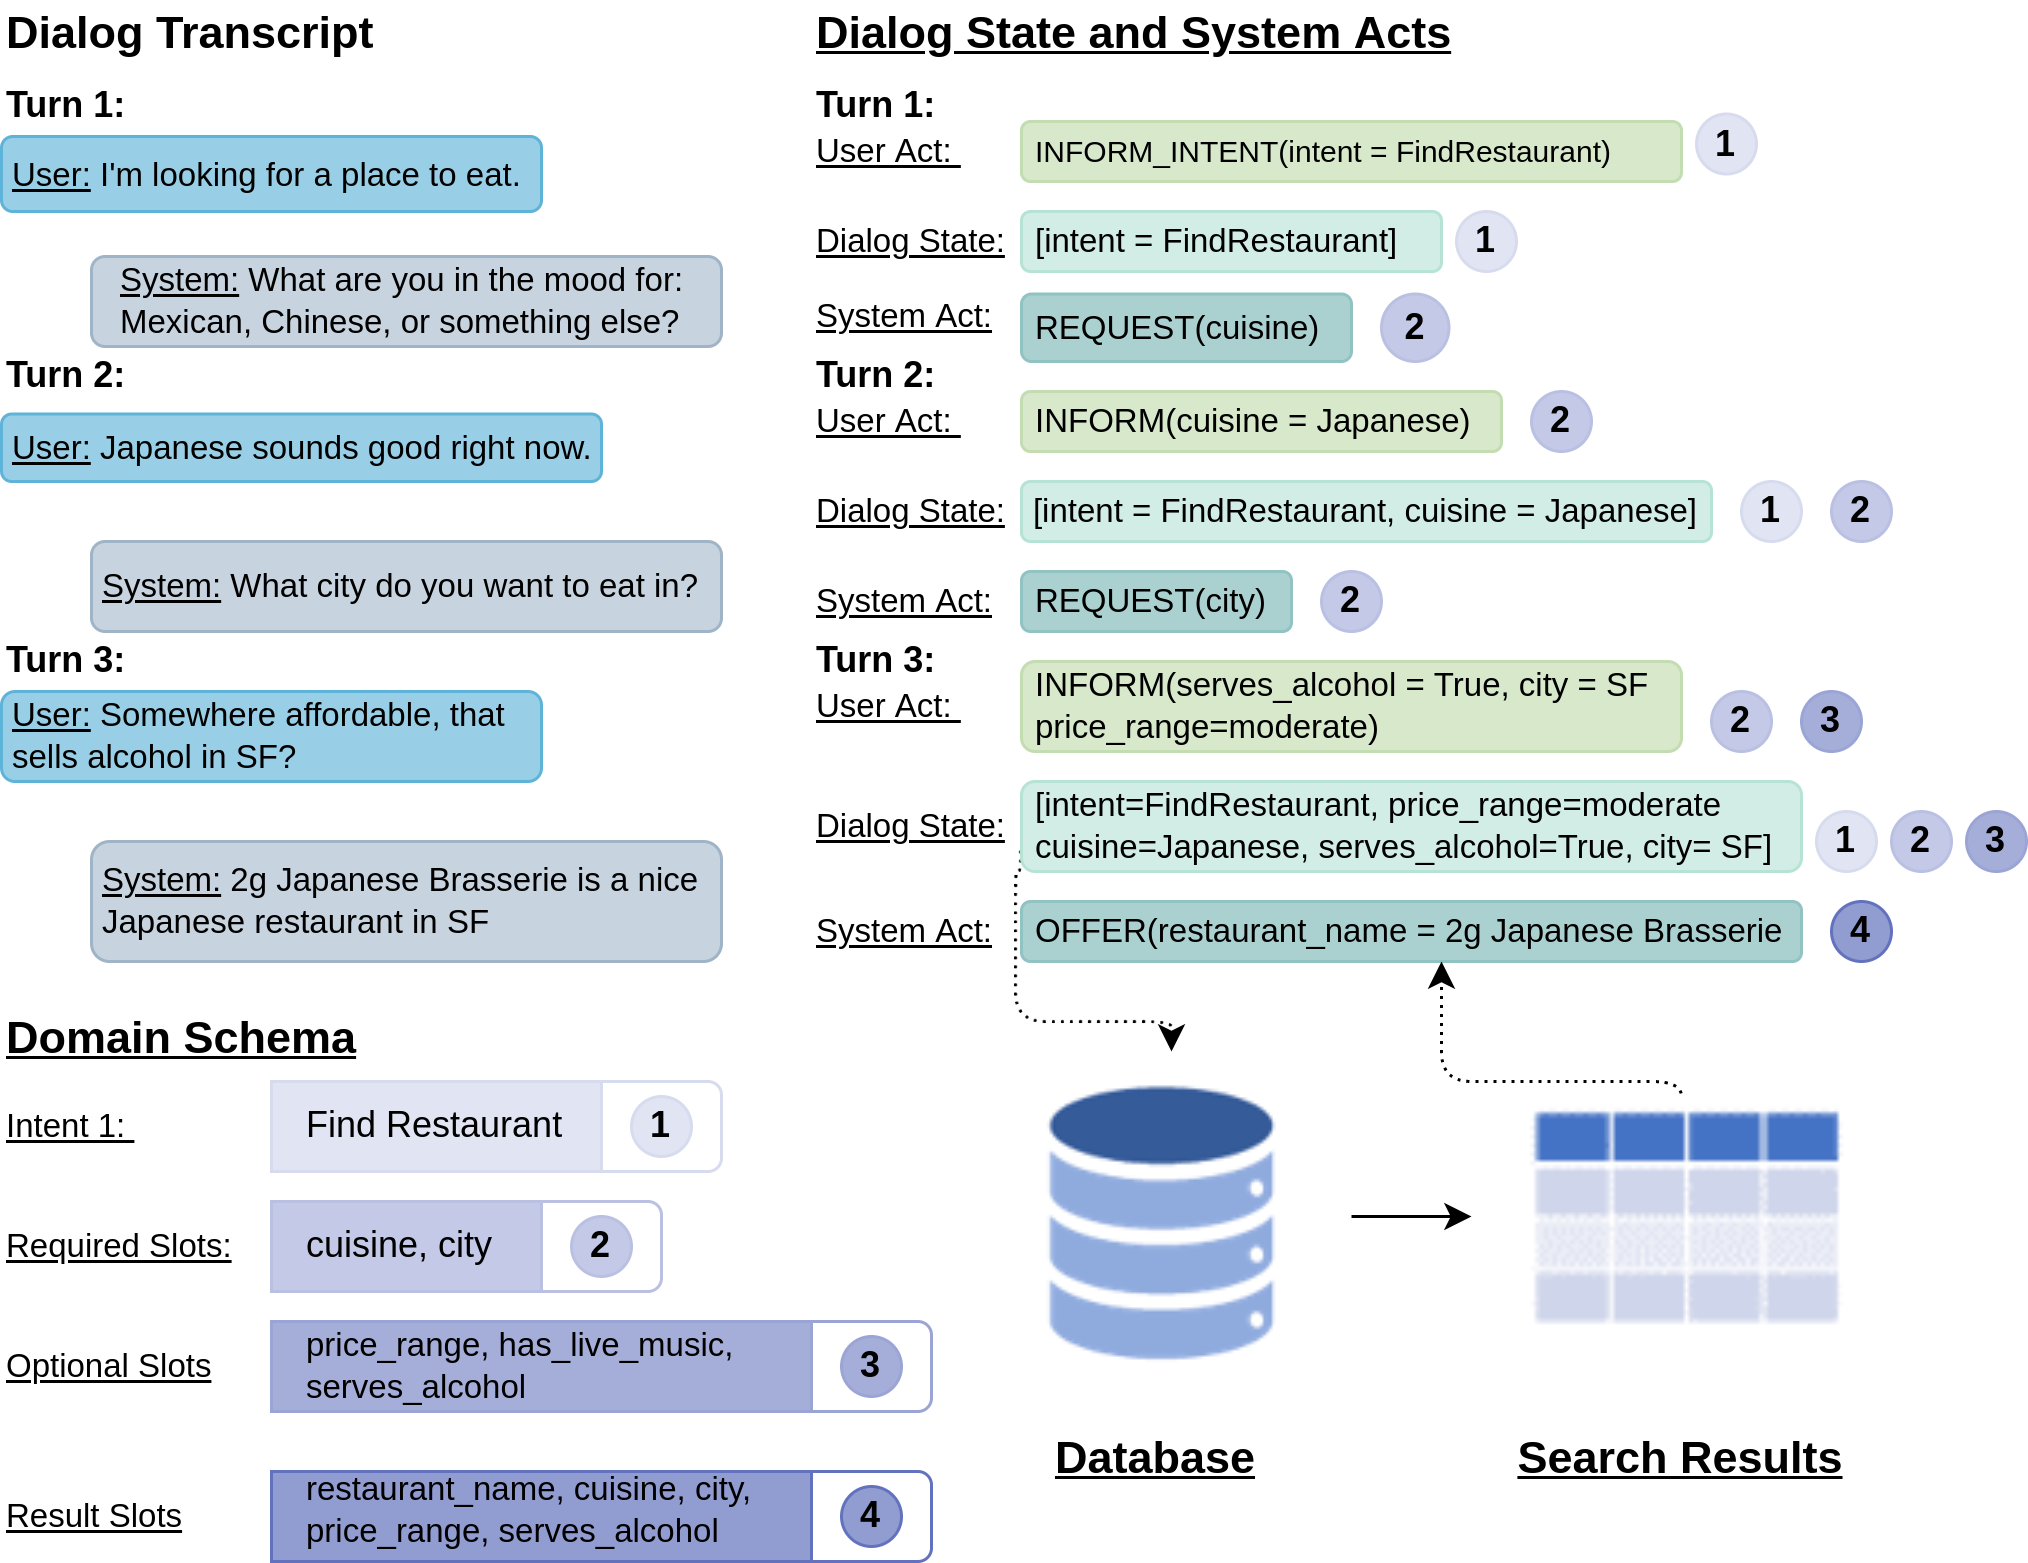
\includegraphics[width=\linewidth]{assets/approach.png}
    \caption{
        Overview of how a Task Oriented System works using schema.
        Given a dialog history consisting of the user and system utterances and the domain schema, for the current turn the dialog state, system actions and system response is generated.
        Parts of the schema that assist in the generation are grouped by similar colors.
    }
    \label{fig:approach}
\end{figure}

\begin{figure*}
    \centering
    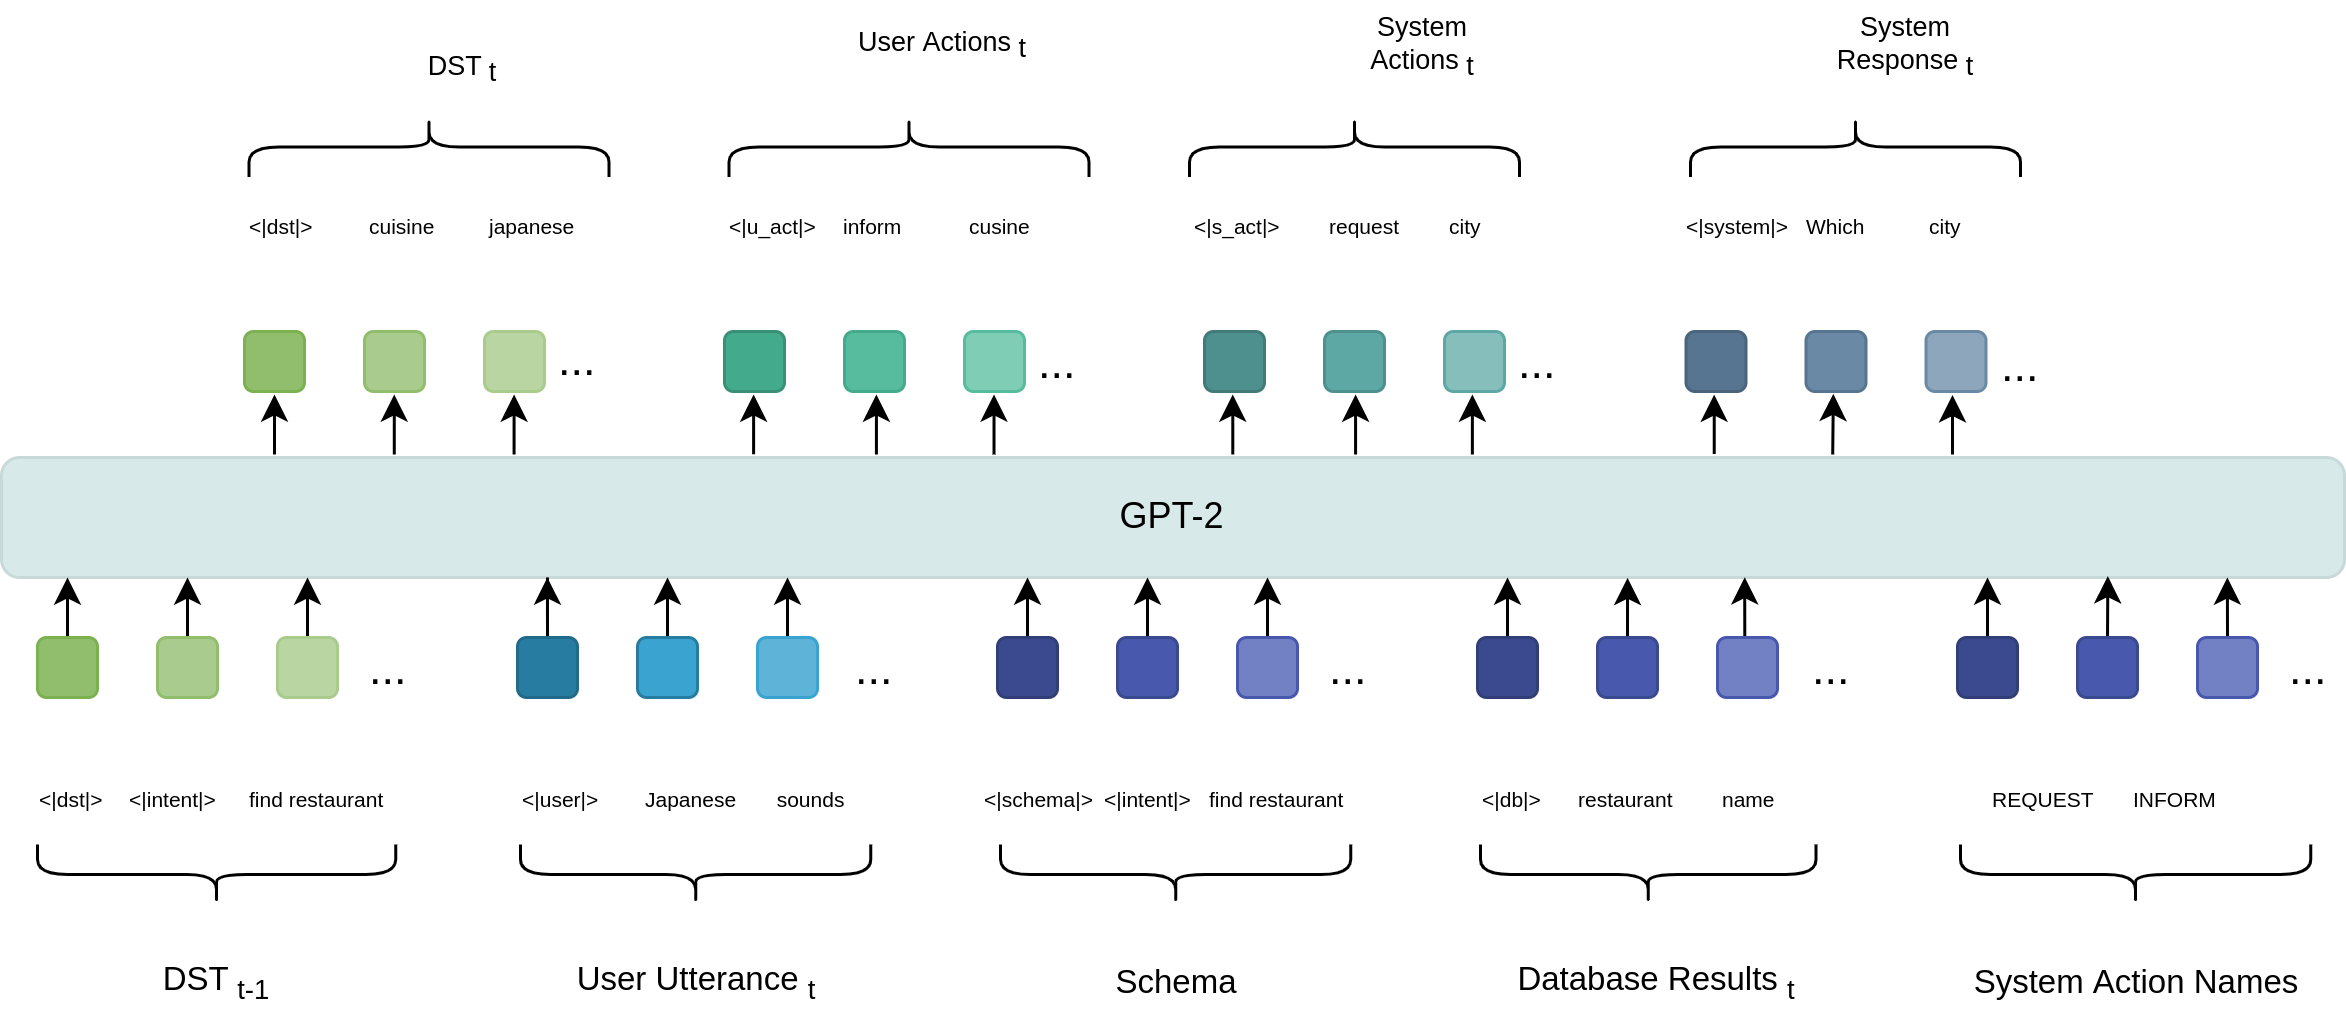
\includegraphics[width=\linewidth]{assets/our_model.png}
    \caption{
        Overview of our approach. A GPT-2 model is fed the dialog state of the previous turn, last user utterance, relevant schemas, database search results and a list of system action names.
        As output, the model autoregressively generates the current dialog state, user actions, system actions and system response.
    }
    \label{fig:our_model}
\end{figure*}

A major drawback of most of these systems is that they fail to generalize to unseen domains. In real-world setting, ideally a model
should have the capablity to adjust to new domains. Domain knowledge in dialoges can be represented by incorporating schema, which
consists of possible intents, slots and slot values. Slot values that have a predefined set of values are labeled a
categorical slot, whereas slot values that can take any value are labeled as a non-categorical slot.
An overview of how a TOD system works by incorporating schema is shown in Figure~\ref{fig:approach}.

Some work has been done to address this issue~\cite{Feng2020ASA,Lee2021DialogueST,Noroozi2020AFA,Mosig2020STARAS,Mehri2021SchemaGuidedPF},
but the focus has been on DST and next action prediction, not end-to-end systems.
Another issue is that in dialogs with many turns, the dialog history becomes very long, repetitive,
and slot values could be updated multiple times in different turns depending on the needs of the user,
thus making it difficult for systems to correctly model long-range semantic dependencies~\cite{sun2022mars}.

To address the aforementioned challenges, we propose a novel Schema Guided Zero-Shot Generalizable End-to-End TOD system using Context Summarization
that outperforms existing state-of-the-art systems.
We use a summarized context consisting of the latest DST, the last user utterance, related domain schemas and system action names.
We also propose a two step training process, where in the first pass we calculate the cross entropy loss on the context and target, and
in the second pass we calculate the loss only on the target. We conduct experiments on the Schema-Guided Dialog~(SGD) dataset
and perform a thorough analysis and an ablation study to show the effectiveness of our approach. To the best of our knowledge,
this is the first Zero-Shot End-to-End TOD system designed for the SGD dataset. \textbf{add sgd-x, long range dependency results}


